\chapter{Weiterentwicklung des Benutzerkonzepts auf Basis der Ergebnisse der Nutzerumfrage}

Basierend auf den Ergebnissen der Nutzerumfrage wird das Benutzerkonzept weiterentwickelt (siehe Abbildung \ref{Bedienungskonzept_V2}). Mehrere Änderungen sind eingebunden, um die Benutzerfreundlichkeit zu verbessern.

\begin{figure}[h]
    \centering
    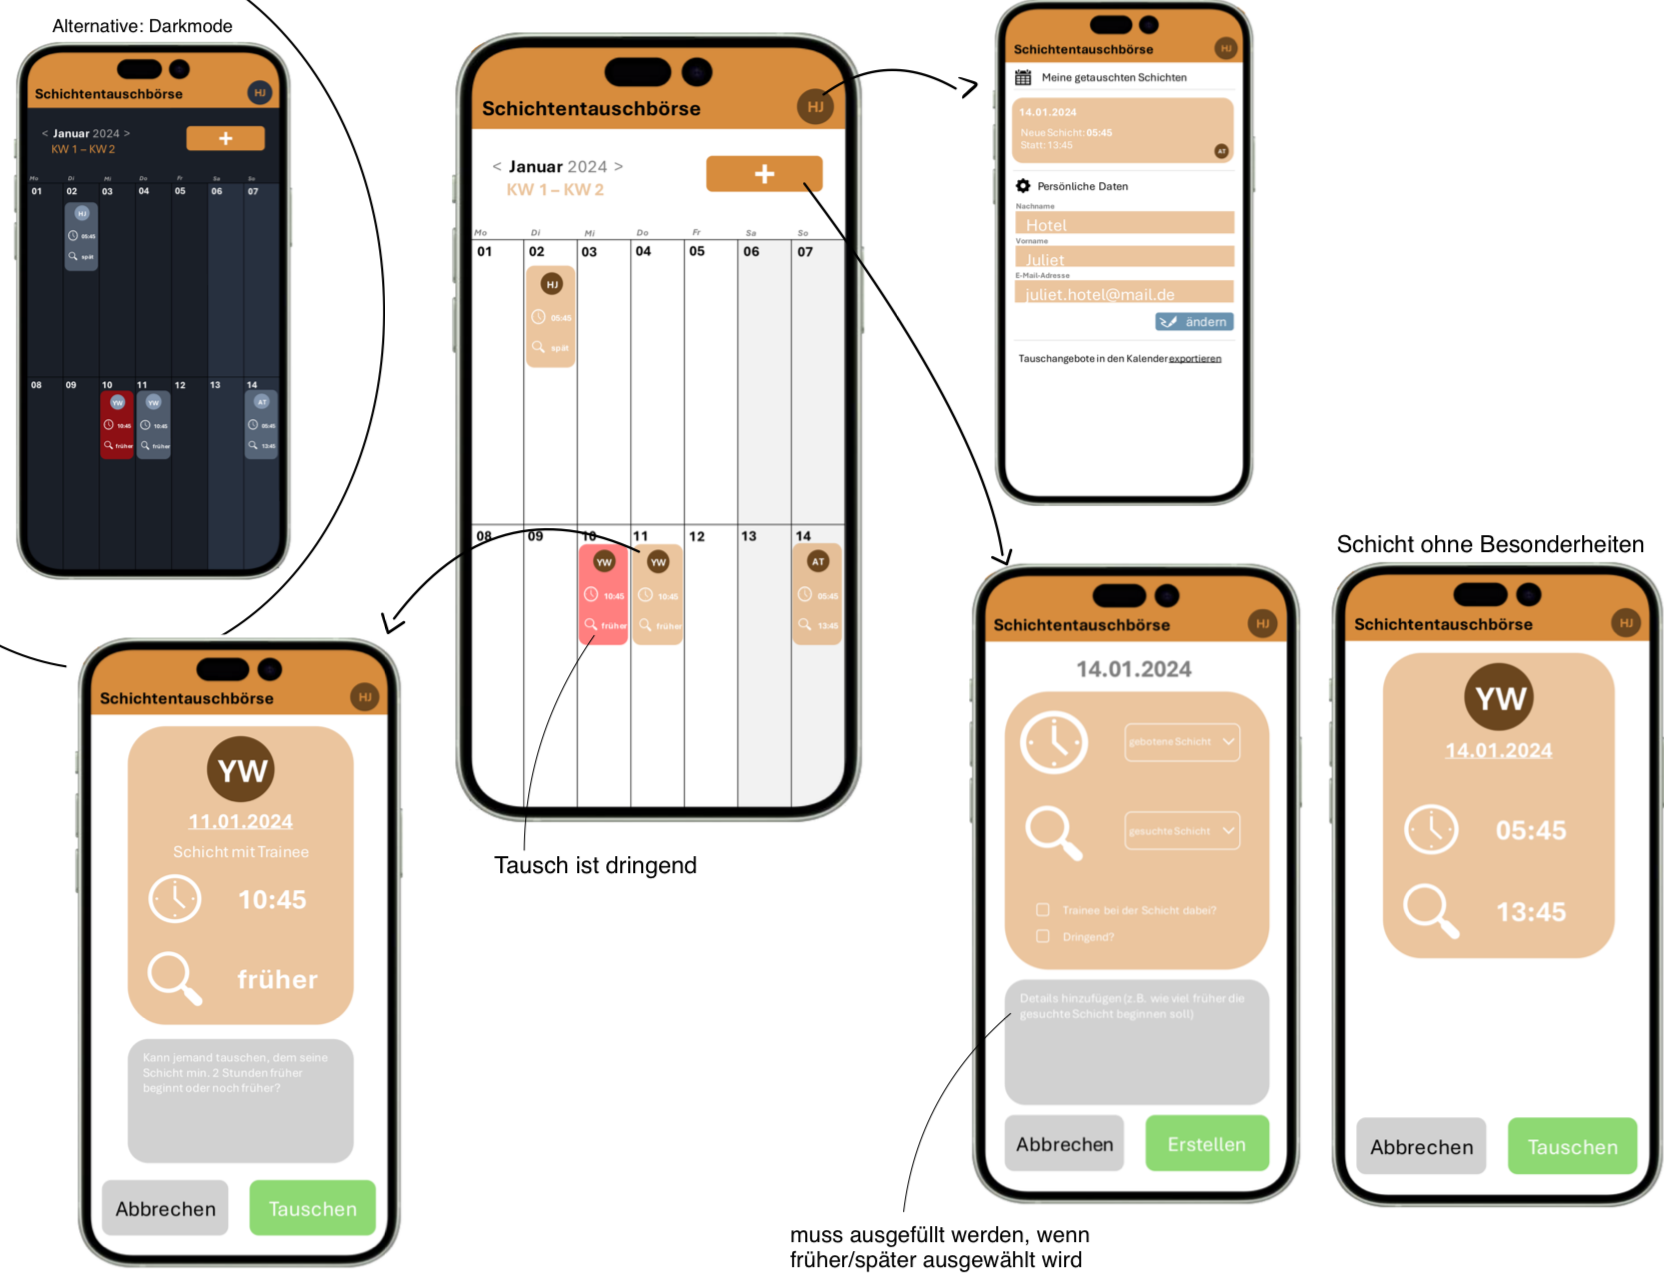
\includegraphics[clip,width=1\linewidth]{images/Bedienungskonzept_V2.png}
    \caption[Weiterentwickeltes Benutzerkonzept]{Weiterentwickeltes Benutzerkonzept (Seite zum Registrieren und zum Einloggen sind gleich geblieben und sind deswegen nicht mit abgebildet)}
    \label{Bedienungskonzept_V2}
\end{figure}

Nutzer haben nun in den Einstellungen die Möglichkeit, Tauschangebote in ihren persönlichen Kalender zu exportieren. Dies erleichtert die Planung und Übersicht ihrer Schichtwechsel.

Außerdem werden Nutzer beim Hinzufügen einer neuen Schicht nach zusätzlichen Details gefragt. Insbesondere wird erfragt, ob ein Trainee bei der Schicht anwesend sein wird oder ob die Anfrage dringend ist. Dringende Anfragen sind visuell hervorgehoben, indem sie rot hinterlegt sind. Dies gilt sowohl im normalen als auch im Dark Mode, wie auf den Übersichtsseiten dargestellt.

Wenn Nutzer im Dropdown-Menü nur „später“ oder „früher“ auswählen, müssen sie einen Kommentar im Kommentarfeld hinzufügen. In anderen Fällen bleibt es den Nutzern überlassen, ob sie zusätzliche Details einfügen möchten.

Unten rechts auf der Abbildung \ref{Bedienungskonzept_V2} ist ein Beispiel für eine Tauschanfrage ohne besondere Merkmale zu sehen. Links neben der Übersichtsseite wird eine Tauschanfrage dargestellt, bei der ein Trainee bei der Schicht anwesend ist und die gesuchte Schicht früher stattfinden soll, mit geschriebenen Details im Kommentarfeld.

Weitere Vorschläge für zusätzliche Informationen aus der Nutzerumfrage wurden protokolliert, jedoch bislang nicht eingebunden.